\documentclass[]{article}

\usepackage[utf8]{inputenc}
\usepackage{fancyhdr} % Required for custom headers
\usepackage{lastpage} % Required to determine the last page for the footer
\usepackage{extramarks} % Required for headers and footers
\usepackage{graphicx} % Required to insert images
\usepackage[spanish]{babel}
\usepackage{url}
\usepackage{package}

\newcommand{\me}{Gabriel De La Parra}
\newcommand{\class}{CC3102 - Teoría de la Computación}
\newcommand{\institution}{Departamento de Ciencias de la Computación\\ \textsc{Universidad de Chile}}
\newcommand{\task}{Tarea 1: Lenguajes Regulares}

\topmargin=-.45in
\evensidemargin=0in
\oddsidemargin=0in
\textwidth=6.5in
\textheight=9.0in
\headsep=0.25in


\pagestyle{fancy}
\lhead{\me} % Top left header
%\chead{\class} % Top center head
\rhead{\task} % Top right header
%\lfoot{\lastxmark} % Bottom left footer
\cfoot{} % Bottom center footer
\rfoot{\thepage\ / \protect\pageref{LastPage}} % Bottom right footer
%\rfoot{Page\ \thepage\ of\ \protect\pageref{LastPage}} % Bottom right footer

% Title Page
\title{\task \\ {\normalsize \class \\ \institution \\}}

\author{\me}
\date{\today}


\begin{document}
	
	\maketitle
	\newpage
	\tableofcontents
	\newpage
	
	
\section{Problema 1}
Para cada una de los siguientes lenguajes, dibuje el diagrama de estados del autómata finito determinista que reconozca el lenguaje. Todos los lenguajes son sobre el alfabeto {0,1}
\\
\subsection{L1 = {w|w no termina en 01}}
\epsilon\varepsilon

\begin{center}
	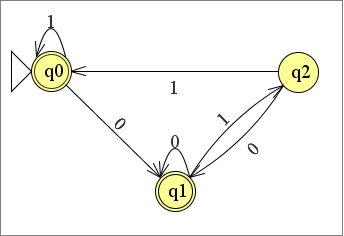
\includegraphics[scale=1]{1A.PNG}
\end{center}

\subsection{L2 = {w|w tiene sólo un substring 101 o comienza con 1 }}

\begin{center}
	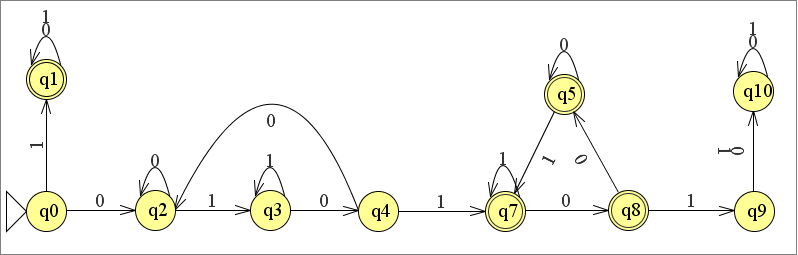
\includegraphics[width=\textwidth]{1B.PNG}
\end{center}

\subsection{L3 = {w|w es tal que tanto el número de 0’s como el número de 1’s es impar \} }

\begin{center}
	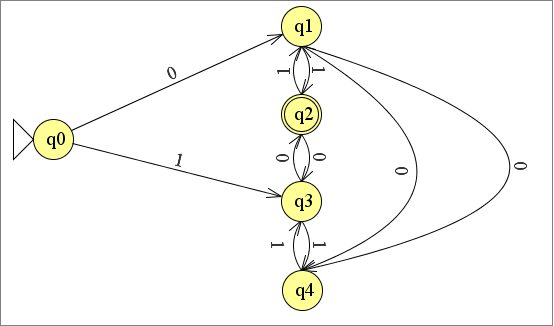
\includegraphics[width=\textwidth]{1C.PNG}
\end{center}

\section{Problema 2}


\end{document}
